\section{Vokselių vizualizavimas}

Galima būtų išskirti dvi vokselių vizualizavimo koncepcijas: tiesiogines ir
netiesiogines.

Netiesioginės – tai tūrinio objekto vertimas į paviršių ir pastarojo
vizualizavimas. Tiesioginės tuo tarpu stengiasi išvengti konvertavimo žingsnio
ir viską atlikti, išlaikant visus tūrinius duomenis.

\subsection{Netiesioginis}

Nepaisant šiandieninių techninių galimybių ir naujovių, poligonai vis dar
gana stipriai dominuoja realaus laiko kompiuterinėje grafikoje (ir
nepanašu, kad ketina užleisti lyderės poziciją). Taigi, vienas iš būdų
atlikti tūrinio objekto vizualizavimą yra pastarojo vertimas į paviršių
ir to paviršiaus vaizdavimas. Tūrinis objektas dalyvauja tik
konvertavimo žingsnyje -- visa kita yra darbas su tų tūrių poligonine
imitacija.

Netiesioginio vizualizavimo pliusai:
\begin{itemize}
\item Poligonai -- vis dar pats populiariausias būdas vizualizuoti realiame laike
\item Pats konvertavimas yra vienkartinis procesas
\end{itemize}

Minusai:
\begin{itemize}
\item Tūrinį objektą konvertavus į paviršių, prarandamas pats tūris
\item Netinka pusiau permatomiems objektams
\item
  Konvertuoti gali tekti ir ne vieną kart -- jeigu tūrinis objektas
  interaktyviai keičiasi pačio vizualizavimo metu
\end{itemize}

\subsection{Žygiuojančių kubų algoritmas}

Žygiuojančių kubų algoritmas (\emph{Marching Cubes}) \cite{bib:marching-cubes}
-- vienas iš bazinių tūrinių duomenų netiesioginių vizualizavimo algoritmų.
Pagrindinė idėja yra imti ir padalinti erdvę į mažus kubelius. Šitas
padalijimas nebūtinai turi sutapti su erdvėje esančiais vokseliais – nei jų
dydžiu, nei jų orientacija. Netgi geriau jeigu nesutaps. Tada keliauti per
kiekvieną iš kubų ir žiūrėti kiek, kurios ir kaip kubų kraštinės kertasi su
duotais vokseliais. Galima atskirti trimatės gardelės viršūnes -- tas, kurios
yra objekto viduje ir tas, kurios yra išorėje. Pagal surinktus susikirtimų
duomenis paskaičiuojamas vokselius aproksimuojantis paviršius (Pav.
\ref{fig:marchingcubes_steps}). Algoritmas kreipia dėmesį tik į tas kraštines,
kurios turi skirtingos kategorijoms priklausančias viršūnes.

\begin{figure}[b]
\centering
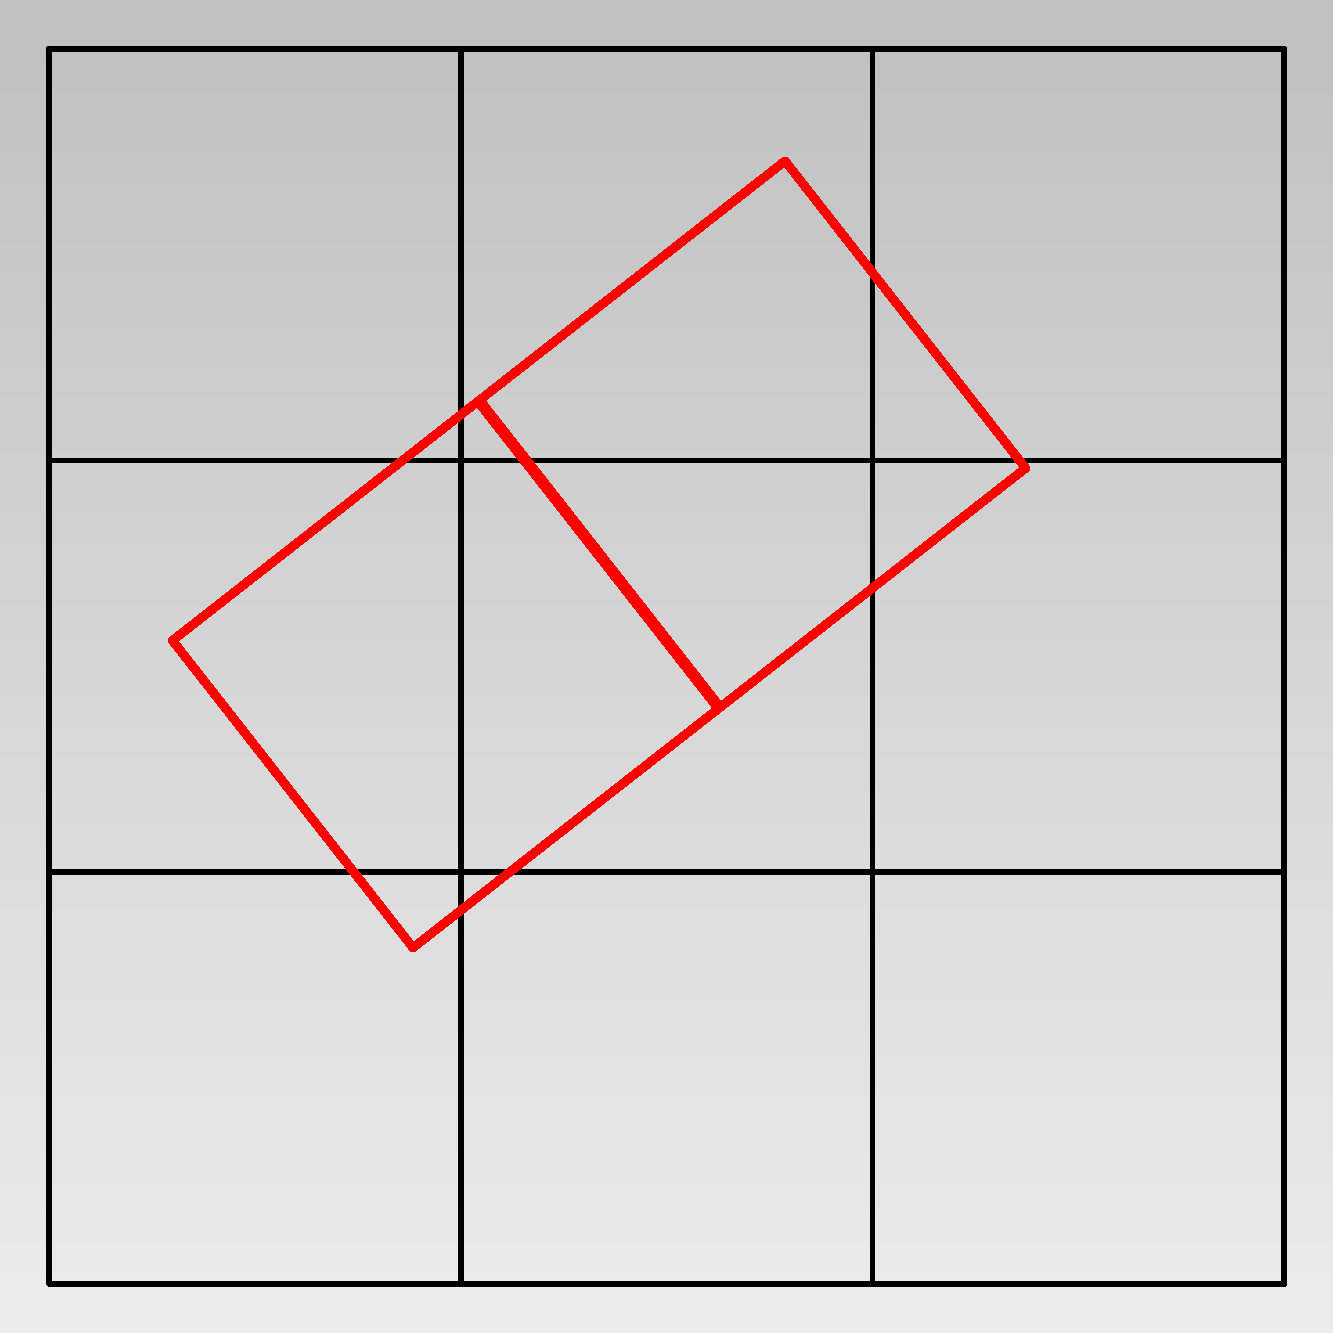
\includegraphics[height=4.5cm]{marching_cubes_step1.pdf}
\includegraphics[height=4.5cm]{marching_cubes_step2.pdf}
\includegraphics[height=4.5cm]{marching_cubes_step3.pdf}
\caption{2D pjūviai: Erdvės padalijimo (juoda) ir vokselių (raudona); Tūrinio
objekto viduje, esančios gardelės viršūnės (oranžinė); Suformuotas paviršius
(mėlyna)}
\label{fig:marchingcubes_steps}
\end{figure}

\subsection{Panaudojant 2D tekstūras}

Tai tiesioginis vizualizavimo būdas. Erdvė yra sukapojama pjūviais
(lygmenimis, diskais) atsisukusiais priekiu į kamerą (Pav.
\ref{fig:2d_tex_layers}). Tada, yra keliaujama nuo galo į priekį sumuojant
spalvines ir permatomumo reikšmes. Galima įvesti šiokį tokį poligonizavimą ir
pjūvius vaizduoti kaip poligo-nus, o jų spalvines ({\em RGBA}) reikšmes kaip
tekstūras (Pav. \ref{fig:2d_tex_camera}). Pagrindinė bėda ta, kad kiekvieną
kartą, pasikeitus apžvalgos kampui, reikia generuoti tiek poligonus, tiek
pačias tekstūras.

\begin{figure}[!ht]
\centering
\includegraphics[height=6.5cm]{2d_tex_layers.png}
\caption{Sumuojant pjūvių reikšmes, gaunamas galutinis vaizdas}
\label{fig:2d_tex_layers}
\end{figure}

\begin{figure}[!ht]
\centering
\includegraphics[height=5.5cm]{2d_tex_90.png}
\includegraphics[height=5.5cm]{2d_tex_45.png}
\caption{Kiekvieną kartą keičiantis apžvalgos kampui, būtina perskaičiuoti
tiek pjūvius, tiek tekstūras}
\label{fig:2d_tex_camera}
\end{figure}

\clearpage

\subsection{Panaudojant 3D tekstūras}

Tai tiesioginis vizualizavimo būdas. Labai primena būdą, naudojant 2D
tekstūras. Tik šiuo atve-ju visi duomenys yra saugomi 3D tekstūroje.
Tada generuojant pjūvius, nebereikia pergeneruoti tekstūros -- užtenka tiesiog
teisingai parinkti pjūvių viršūnių tekstūrų koordinates. Kadangi nereikia
generuoti tekstūrų, tai ir įvairius tarpinius duomenų nuskaitymo žingsnius
(tokius kaip interpoliacija) galima palikti aparatūrinei įrangai ir/ar
grafinėms bibliotekoms.

\subsection{Tūrinis spindulių skleidimas}

Pagrindinė tūrinis spindulių skleidimo  (\emph{Ray Casting}. Pav.
\ref{fig:ray_casting}) idėja šiek tiek primena spindulių trasavimo (\emph{Ray
Tracing}) algoritmą. Spindulys yra skleidžiamas iš kameros pozicijos į sceną,
susidedančią iš tūrinių objektų. Spindulio kelionės metu, kaupiama fragmento
spalvų ir permatomumo reikšmės. Tačiau, kitaip nei spindulių trasavime,
procedūra nėra rekursyvi.

\begin{figure}[!ht]
\centering
\includegraphics[height=8.0cm]{ray_casting}
\caption{Tūrinis spindulių skleidimas.}
\label{fig:ray_casting}
\end{figure}

